\section{Theorie}
\label{sec:Theorie}

\subsection {Gedämpfte Schwingungen}
Besteht ein Schaltkreis aus einer Induktivität $L$, realisiert durch eine Spule, und einem Kondensator mit der Kapaziät $C$, führt das System
ungedämpfte Schwingungen durch. Die Energie pendelt zwischen den Speichern hin und her und führt deshalb periodische Schwingungen durch.
Wird dem Schaltkreis ein ohmscher Widerstand $R$ hinzugefügt, nimmt die Energie mit der Zeit ab, die Amplituden von Strom und Spannung fallen,
und das System führt Gedämpfte Schwingungen aus. Ein Aufbau eines solches Schwingkreises ist in Abbildung (1) dargestellt. Dieses System führt
\begin{figure}[H]
  \centering
  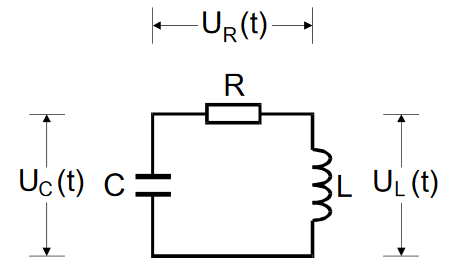
\includegraphics[height=5cm]{RLC.png}
  \caption{Aufbau eins RLC-Schwingkreises. \cite[S.1]{kent}}
\end{figure}
Mit Hilfe des 2. Kirchhoffschen Gesetzes kann man die Differentialgleichung für den Schaltkreis aufstellen.
\begin{equation}
U_R (t) + U_C (t) + U_L (t) = 0 .
\end{equation}
Setzt man die Gleichungen
\begin{align}
U_R (t) = R I(t)  \\
U_C (t) = \frac{Q(t)}{C}  \\
U_L (t) = L \frac{dI}{dt} \\
I = \frac{dQ}{dt}
\end{align}
mit $Q(t)$ als Ladung in die DGL ein, und leitet einmal ab, ergibt sich 
\begin{equation}
\frac{d^2I}{dt^2} + \frac{R}{L}\frac{dI}{dt} + \frac{1}{LC}I = 0 .
\end{equation}

